% !TEX encoding = UTF-8 Unicode
% $Header: /cvsroot/latex-beamer/latex-beamer/solutions/generic-talks/generic-ornate-15min-45min.en.tex,v 1.5 2007/01/28 20:48:23 tantau Exp $

\documentclass{beamer}
\usepackage[brazil]{babel}
\usepackage[T1]{fontenc}
%\usepackage[latin1]{inputenc}
\usepackage[utf8]{inputenc}
\usepackage[ruled,linesnumbered,vlined,boxed]{algorithm2e} %pacote para formatar algoritmos
%\usepackage[cmex10]{amsmath}

% This file is a solution template for:

% - Giving a talk on some subject.
% - The talk is between 15min and 45min long.
% - Style is ornate.



% Copyright 2004 by Till Tantau <tantau@users.sourceforge.net>.
%
% In principle, this file can be redistributed and/or modified under
% the terms of the GNU Public License, version 2.
%
% However, this file is supposed to be a template to be modified
% for your own needs. For this reason, if you use this file as a
% template and not specifically distribute it as part of a another
% package/program, I grant the extra permission to freely copy and
% modify this file as you see fit and even to delete this copyright
% notice. 


\mode<presentation>
{
  \usetheme{Warsaw}
  % or ...

  \setbeamercovered{transparent}
  % or whatever (possibly just delete it)
}

%\usepackage[english]{babel}
%\usepackage[brazil]{babel}
% or whatever

%\usepackage[latin1]{inputenc}
% or whatever

\usepackage{times}
%\usepackage[T1]{fontenc}
% Or whatever. Note that the encoding and the font should match. If T1
% does not look nice, try deleting the line with the fontenc.

\usepackage{moreverb} 
\usepackage{verbatim}

\usepackage{hyperref}

%\title[Short Paper Title] % (optional, use only with long paper titles)
\title[Projeto Final] % (optional, use only with long paper titles)
{Camadas de Acessso ao Meio para Redes de Sensores Sem Fio}

%\subtitle
%{Uma solução voltara para reuso e confiabilidade} % (optional)

\author[hugo] % (optional, use only with lots of authors)
{Hugo Braga\\
Orientador: Proof. Flávio Assis
}
% - Use the \inst{?} command only if the authors have different
%   affiliation.

\institute[UFBA] % (optional, but mostly needed)
{
  Especialização Avançada em Sistemas Distribuídos\\
  Universidade Federal da Bahia}
% - Use the \inst command only if there are several affiliations.
% - Keep it simple, no one is interested in your street address.

\date[Short Occasion] % (optional)
{24 de Fevereiro de 2011 / Projeto Final}

\subject{Talks}
% This is only inserted into the PDF information catalo-. Can be left
% out. 



% If you have a file called "university-logo-filename.xxx", where xxx
% is a graphic format that can be processed by latex or pdflatex,
% resp., then you can add a logo as follows:

% \pgfdeclareimage[height=0.5cm]{university-logo}{university-logo-filename}
% \logo{\pgfuseimage{university-logo}}



% Delete this, if you do not want the table of contents to pop up at
% the beginning of each subsection:
%\AtBeginSubsection[]
%{
%  \begin{frame}<beamer>{Outline}
 %   \tableofcontents[currentsection,currentsubsection]
 % \end{frame}
%}


% If you wish to uncover everything in a step-wise fashion, uncomment
% the following command: 

%\beamerdefaultoverlayspecification{<+->}

\begin{document}

\begin{frame}
  \titlepage
\end{frame}

\begin{frame}{Estrutura da apresentação}
  \tableofcontents
  % You might wish to add the option [pausesections]
\end{frame}


% Since this a solution template for a generic talk, very little can
% be said about how it should be structured. However, the talk length
% of between 15min and 45min and the theme suggest that you stick to
% the following rules:  

% - Exactly two or three sections (other than the summary).
% - At *most* three subsections per section.
% - Talk about 30s to 2min per frame. So there should be between about
%   15 and 30 frames, all told.
%\section{Introdução}
%\begin{comment}
\begin{frame}{Resumo}
  Estudo do estado-da-arte dos protocolos de Camada de Acesso ao Meio (MAC) para Redes de Sensores sem Fio (RSSF), apresentando uma classificação e destacando os 
principais protocolos além de destacar as características inovadoras dos protocolos nos últimos anos bem como alguns protocolos que as possuem.
\end{frame}
%\end{comment}


%\subsection[pequeno titulo]{Motivação}
%\subsection[Motivação]{Motivação}

\section{Introdução}
\subsection{RSSF}
\begin{frame}{Redes de Sensores sem Fio}
  % - A title should summarize the slide in an understandable fashion
  %   for anyone how does not follow everything on the slide itself.
  \begin{itemize}
    \item
      Redes de Sensores sem Fio (RSSF) são formadas por nós caracterizados pela limitação dos recursos.
    \item
      Utilizada para sensoriar e colher dados relacionados a alguma grandeza física.
      \begin{itemize}
       \item Monitoração de regiões remotas.
	\item Monitoração da saúde das pessoas.
	\item Aplicações militares.
      \end{itemize}
  \item
    Conservação de energia é um fator importante em Redes de Sensores sem Fio (RSSF).
    \begin{itemize}
    	\item
    		Limitação dos recursos energéticos.
    	\item
    		Troca de bateria em alguns casos é inviável.
    \end{itemize}
  \end{itemize}
\end{frame}

\subsection{MAC}
\begin{frame}[allowframebreaks]{Protocolos de Camadas de Acesso ao Meio}
  \begin{itemize}
    %\item Arquitetura dos nós sensores composta por: unidade de processamento, memória, sensores, rádio e fonte de energia.
    \item
      Unidade de comunicação (rádio) corresponde ao elemento de maior consumo energético.
    \item
      Camada de acesso ao meio (MAC) consiste na principal forma de influenciar o rádio, tendo em vista à redução do consumo energético.
      \begin{itemize}
       \item Define quem e quando terá acesso ao meio físico para realizar a comunicação.
      \end{itemize}
    \item
      Em quase todos os trabalhos estudados, a redução energética é objetivo primordial, exceto em \cite{20093812310364}.
    \item
      As principais formas de gasto energético são:
      \begin{itemize}
       \item escuta ociosa (\emph{idle listening}).
	\item colisão.
	\item \emph{overhearing}.
	\item sobrecarga (\emph{overhead}) das mensagens de controle.
      \end{itemize}
  \end{itemize}
\end{frame}


\section{Classificação}
\begin{frame}{Classificação}
  \begin{itemize}
    \item
      Os protocolos (para MACs) podem ser classificados em \cite{kredo07}:
	\begin{itemize}
	  \item Baseados em escalonamento.
	  \item Baseados em acesso aleatório.
	\end{itemize}
    \item Uma outra classificação divide os protocolos em: baseados em TDMA, baseados em contenção e protocolos multicanais \cite{20084511683228}.
    \item Procurou-se adotar uma mescla das duas classificações, adicionando a classe dos multicanais à primeira classificação.
  \end{itemize}
\end{frame}

\subsection{Baseados em escalonamento}

\begin{frame}{Protocolos baseados em escalonamento}

  \begin{itemize}
  \item
    Organizam o meio físico dividindo-o em \emph{slots} (de tempo, de frequência ou de código).
  \item
    Tradicionalmente, a opção por este tipo de protocolo pretente evitar colisões, \emph{idle listening} e \emph{overhearing}.
  %\item Protocolos sincronizados não necessariamente são baseados em escalonamento $\rightarrow$ S-MAC.
  %\item
  %  Divisão em \emph{slots} não implica em que colisões (além de \emph{idle listening} e \emph{overhearing}) não ocorrerão.
  %    \begin{itemize}
  %	\item Em \cite{20102813064978}, a comunicação dentro de cada \emph{slot} se dá através de contenção.
  %	%um numero menor de nos vao disputar o meio pois os nos sao divididos em clusters e o slot diferente eh atribuido para cada cluster
  %	\item Em \cite{20083811560517}, \emph{slots} de dados (livre de contenção) podem se transformar em \emph{slots} de controle (com contenção).
  %	\item Protocolos que explicitam a necessidade e vantagem da utilização de ambas as abordagens serão considerados híbridos.
  %    \end{itemize}
  \item
    Podem ser divididos em dois tipos:
      \begin{itemize}
	\item distribuído.
	\item centralizado.
      \end{itemize}
  \end{itemize}
  
\end{frame}

\begin{frame}{Distribuído}
\hypertarget{cws-mac_back}{}
  \begin{itemize}
    \item A tarefa de distribuir as mensagens de sincronização e definir o momento em que cada um pode se comunicar é feita de maneira distribuída.
    \item Em \cite{20083811560517} é apresentado o protocolo híbrido \emph{Cooperative Wireless Sensor Medium Access Control} (CWS-MAC) \hyperlink{cws-mac}{\beamergotobutton{Quadro}}.
    \begin{itemize}
      \item Objetiva atender tanto aos requisitos das mensagens de controle como das mensagens de dados.
      \begin{itemize}
	\item Mensagens de dado: periódicas, requisitam largura de banda e são tolerantes à descartes $\rightarrow$ escalonadas.
	%As mensagens de dados por requisitarem grande largura de banda, sao transmitidos de forma escalonada
	\item Mensagens de controle: curtas, não toleram descartes e necessitam de mínimo atraso (diferente de atraso determinístico) $\rightarrow$ mini-slots com contenção.
	%para um no roubar um quadro de dado, ele informa no beacon que quer enviar uma msg de controle. Antes de transmitir a mensagem de dado, caso o no 
	%que detem o slot escutar o beacon, ele cede espaco para o no do beacon transmitir msg de controle. O slot de dado eh transformado em varios mini-slots de controle
	% e o acesso a estes mini-slots eh feita de forma aleatoria (com contencao). Para garantir a entrega, ACKs sao utilizados
      \end{itemize}
      \item
	Atraso: quadro de controle pode 'roubar' quadro de dado.
    \end{itemize}
  \end{itemize}
\end{frame}

\begin{frame}[allowframebreaks]{Centralizado}
\hypertarget{aerial_back}{}
  \begin{itemize}
    \item A tarefa de sincronização e de definição de escalonamento é realizada por um único nó.
    \begin{itemize}
      \item Em \cite{20100312645920} é proposto um protocolo que utiliza uma plataforma aérea para auxiliar na execução de duas atividades: \hyperlink{aerial}{\beamergotobutton{Plat.}}.
      \begin{itemize}
	\item Coordenação centralizada: dispositivo captura informações de topologia, definindo escalonamento dos nós além dos melhores caminhos para as mensagens.
	\item Transmissão direta: elimina protocolo de roteamento e comunicação \emph{multi-hop} $\rightarrow$ em fator de decaimento do sinal na comunicação aérea é menor do que 
  na comunicação terrestre.
      \end{itemize}
      \item Para dar suporte às duas funcionalidades, dois protocolos são propostos:% \hyperlink{quadro_aerial}{\beamergotobutton{Quadro}}:
      \hypertarget{quadro_aerial_back}{}
      \begin{itemize}
	\item \emph{Aerial Platform based Routing and Medium Access Control} (APRMAC): define para cada nó e em cada \emph{slot} de tempo, o estado em que o nó deve estar.
	\item \emph{Aerial Platform MAC} (APMAC): organiza para que cada nó transmita a mensagem livre de colisão, além de se adaptar ao tráfego.
      \end{itemize}
    \end{itemize}
  \end{itemize}
\end{frame}


\subsection{Baseados em acesso aleatório}
\begin{frame}{Protocolos baseados em acesso aleatório}
  \begin{itemize}
    \item O acesso ao meio não é regulado e ocorre sob-demanda.
    \item Protocolos são extensíveis, visto que não existe o \emph{overhead} da coordenação.
    \item Podem ser divididos em dois tipos:
      \begin{itemize}
	\item Síncrono.
	\item Assíncrono.
      \end{itemize}
  \end{itemize}
\end{frame}

\begin{frame}{Síncrono}
  \begin{itemize}
    \item Mecanismo de sincronização entre os nós são adotados $\rightarrow$ permite aos nós tomarem conhecimento do escalonamento dos nós vizinhos.
    %\item Em \cite{Yadav08} é proposto um protocolo que consiste numa variação do S-MAC.
    %  \begin{itemize}
    %	\item Tem por objetivo a eficiência energética e latência.
%	\item Mensagens de sincronização e de RTS foram convertidas em um único pacote $\rightarrow$ redução da latência.
%	\item Nó se adapta ao tráfego variando o \emph{duty cycle}.
	%a medida que o numero de msgs na fila aumenta e passa um threshold, duty cycle duplica. A medida que diminui e fica abaixo do threshold, duty cycle
	% diminui pela metade
 %     \end{itemize}
    \item Em \cite{20102012936055} é proposto um protocolo que consiste numa variação do SMAC.
      \begin{itemize}
	\item Tem por objetivo reduzir o \emph{idle listening}.
	\item Varia o tamanho da janela de contenção (CW) (não se adapta ao tráfego) $\rightarrow$ reduz \emph{idle listening}.
	%trafego menos intenso, probabilidade de colisao menor -> logo o valor de CW pode ser menor, reduzindo energia
	%trafego mais intenso, probabilidade de colisao maior -> logo o valor de CW pode ser maior
      \end{itemize}
  \end{itemize}
\end{frame}

\begin{frame}{Assíncrono}
  \begin{itemize}
    \item Mecanismo de sincronização não são trocadas.
    \item Em \cite{20093112234782} é proposto o protocolo \emph{Game-theoretic} (G-MAC).
      \begin{itemize}
	\item Tem por objetivo garantir vazão e mínimo atraso.
	\item Motivam para o fato de que aplicações começam a ter requisitos de tempo-real.
	\item Vazão e atraso são otimizados levando em consideração restrições energéticas.
	\item Modela o problema de otimização como um jogo cooperativo incompleto.
	\item Não há troca de estados.
	\item A estratégia de cada jogador é ajustada pelo estado (de contenção) do meio.
	%o estado do meio consiste na quantidade de jogadores disputando o acesso ao meio. Esta quantidade eh estimada atraves da probabilidade de transmitir e colisao
	%\item G-MAC divide o tempo em super-quadros, formados por parte ativa e inativa* \hyperlink{quadro_g-mac}{\beamergotobutton{Super-Frame}}.
	\hypertarget{quadro_g-mac_back}{}
      \end{itemize}
  \end{itemize}
\end{frame}

\subsection{Multicanais}
\begin{frame}{Protocolos Multicanais}
  \hypertarget{cmac_back}{}
  \begin{itemize}
    \item Utilizam mais de um canal para transmitirem as mensagens de controle e de dados.
    \item Em \cite{20084511683228} é proposto o CMAC.
    \begin{itemize}
      \item Motiva para o avanço do \emph{hardware}.
      %\item Objetivo principal é reduzir o \emph{idle listening} (consideram como sendo a principal fonte de gasto energético).
      \item Nó equipado com dois rádios:
      \begin{itemize}
	\item Baixo consumo (LR):Possui funções reduzidas, sendo responsável por enviar e receber mensagens de controle.
	\item Robusto (MR): Transmite os dados em qualquer canal.
      \end{itemize}
      \item Três tipos de mensagens são trocadas: \emph{REQ}, \emph{CON} e \emph{WAIT}.
      \item A comunicação ocorre em duas fases: fase de negociação e fase de transmissão do dado \hyperlink{cmac}{\beamergotobutton{Msgs.}}.
      \item A comunicação do dado é feita livre de colisão.
    \end{itemize}
  \end{itemize}
\end{frame}

\section{Características Inovadoras}
\subsection{Mobilidade}
\begin{frame}{Mobilidade}
  \begin{itemize}
    \item Apenas um protocolo foi encontrado que fornece suporte à mobilidade.
    \item Em \cite{20103113115754} é proposto o \emph{Mobile Cluster} MAC (MCMAC).
    %eles referencial o metodo de sincronizacao descentralizada
    %o metodo de alocacao de slots eh utilizado de um outro trabalho que eles apenas citam
    \begin{itemize}
      \item Suporta mobilidade de \emph{cluster} de nós.
      \item Motivam para aplicações da área de saúde: monitoração de pessoas idosas $\rightarrow$ \emph{Wireless Body Area Network} (WBAN).
      \item Neste cenário, existem dois tipos de rede: móvel (WBAN) e fixas.
      \item O quadro é dividido em duas partes: ativo e inativo. A parte ativa é dividida em duas partes \hyperlink{mcmac}{\beamergotobutton{Quadro}}:
	\hypertarget{mcmac_back}{}
	\begin{itemize}
	  \item \emph{Static Active Slots} (SAS).
	  %nos estaticos escutam os o MCS para receber informacoes da WBAN. Durante este periodo, os nos estaticos apenas recebem msgs.
	  \item \emph{Mobile Cluster Slots} (MCS).
	  %nos moveis escutam o SAS para receber informacoes do no sink (atraves da rede estatica) como alarmes, alem das msgs de sincronizacao. 
	  %Durante este periodo, os nos moveis apenas recebem msgs.
	  %Clusters que estejam proximos podem incorrer em colisao (transmissao no mesmo slot). Por isso, dentro de cada slot do MCS existe um periodo para o CSMA.
	  %Mesmo assim pode ocorrer colisao na mudanca do periodo do CSMA para o Tx.
	\end{itemize}
    \end{itemize}
  \end{itemize}
\end{frame}

\subsection{Projeto Cross-Layer}
\begin{frame}{Projeto \emph{Cross-Layer}}
  \hypertarget{macari_tree_back}{}
  \begin{itemize}
	\item Possuem a característica de extrapolar a região que lhe concerne.
	\begin{itemize}
	  \item Obter informações de outras camadas.
	  %Como tratar os pacotes de cada aplicacao
	  \item Elimina protocolo de roteamento.
	  %seja porque o mesmo ja faz o trabalho como no caso da APRMAC, seja porque a rota eh fixa para uma determinada topologia
	\end{itemize}
	\item Em \cite{20092812183087} é proposto o MaCARI.
	\begin{itemize}
	  \item Elimina o protocolo de roteamento em decorrência da topologia fixa \hyperlink{macari_tree}{\beamergotobutton{Árv.}}.
	  \item Período dividido em três fases:
	  \begin{itemize}
	    \item Sincronização.
	    %durante este periodo os nos (coordenadores e nos fins) recebem informacoes para compartilhar uma visao global. Uma ordem global eh imposta
	    %pelo PAN coordinator para que coordenador repasse o beacon sem colisao
	    \item Período escalonado.
	    %durante este periodo, a comunicacao entre um coordenador e seu pai eh feita de forma exclusiva (colision-free).
	    %o ciclo de atividade em cada estrela eh dividida em duas fases: (i)o coordenador coleta informacao do seu sensor e do sensor dos seus filhos (nos fins)
	    %(ii) o coordenador envias as informacoes para o coordenador pai e recebe informacoes dele.
	    \item Período não-escalonado.
	  \end{itemize}
	\end{itemize}
  \end{itemize}
\end{frame}

\subsection{Controle de Potência}
\begin{frame}{Protocolos com controle de potência}
  \begin{itemize}
    \item Em \cite{20094212373426} é apresentado o C-MAC.
    \begin{itemize}
      \item Explora transmissões concorrentes.
      \item Mostram que existe uma relação entre o PRR e o SINR.
      \item Otimiza vazão mesmo na presença de interferência.
      \item Estima pela relação acima o melhor momento e a melhor potência de transmissão (sem CSMA).
    \end{itemize}
  \end{itemize}
\end{frame}

\subsection{Dinamicidade}
\begin{frame}{Dinamicidade}
  \begin{itemize}
    \item Capacidade de variar o \emph{duty cycle} e/ou tempo de ciclo do quadro $\rightarrow$ adaptar-se ao tráfego.
    \item Permite o aumento da vazão assim como redução do atraso.
    \item Em \cite{20100812725891} é proposto o \emph{Fuzzy Logic-based Adaptative Listen for Medium Access Control} (FLAMAC).
    \begin{itemize}
      \item Visa a reduzir o \emph{idle listening}.
      \item Varia o tempo de ciclo.
      \item Baseado em lógica \emph{fuzzy} $\rightarrow$ baixo poder computacional e problema modelado como sistema de controle.
      %dado a energia corrente e o tráfego atual, tomam a decisão para mudar o tempo de ciclo
    \end{itemize}
    %\item Em \cite{20101312811704}, os autores também adotam lógica \emph{fuzzy} para ajustar o momento da difusão de mensagens de escalonamento.
    %quando muitas mensagens estao sendo perdidas em decorrencia do desvio do relogio eh necessario encurtar a periodicidade da divulgação do escalonamento.
  \end{itemize}
\end{frame}

\section{Objetivos}
\begin{frame}{Objetivos Visados}
  \hypertarget{eq-mac_back}{}
  \begin{itemize}
    \item Além de energia, os trabalhos têm visados a vazão, atraso e aumento da razão de entrega das mensagens.
    %\item Em alguns trabalhos, estes objetivos são secundários enquanto em outros eles são considerados principais, ao lado de energia, numa solução de compromisso.
    \item Em \cite{20092612148942} é proposto o EQ-MAC.
    \begin{itemize}
      \item Tem por fim reduzir o consumo energético e prover QoS através da adoção de \emph{Serviços Diferenciados}.
      \item É formado por dois componentes \hyperlink{eq-mac}{\beamergotobutton{Componentes}}:
      \begin{itemize}
	\item \emph{Classifier MAC} (C-MAC): faz a classificação do tráfego.
	\item \emph{Channel Access} (CA-MAC): utiliza acesso aleatório para as mensagens de controle e período escalonado para as mensagens de dado.% \hyperlink{quadro_eq-mac}{\beamergotobutton{Quadro}}.
	\hypertarget{quadro_eq-mac_back}{}
      \end{itemize}
    \end{itemize}
  \end{itemize}
\end{frame}

\section{Considerações Finais}
\begin{frame}{Considerações Finais}
  \begin{itemize}
    \item Protocolos MAC continuam sendo bastante pesquisados $\rightarrow$ por volta de 35 resultados nos últimos 3 anos (sem variar palavras-chave).
    \item Optado por soluções híbridas.
    \item Soluções buscam adaptar-se ao tráfego.
    \item Soluções cross-layer além de comunicação concorrente têm sido levado em consideração.
    \item O suporte à mobilidade ainda não está tendo a devida atenção.
    \item Não apenas energia, mas QoS (atraso e vazão) tem se tornado objetivos principais.
  \end{itemize}
\end{frame}

\begin{frame}
  Dúvidas ?
\end{frame}

\begin{frame}{Quadro do CWS-MAC \cite{20083811560517} \hyperlink{cws-mac_back}{\beamergotobutton{Voltar}}}
\hypertarget{cws-mac}{}
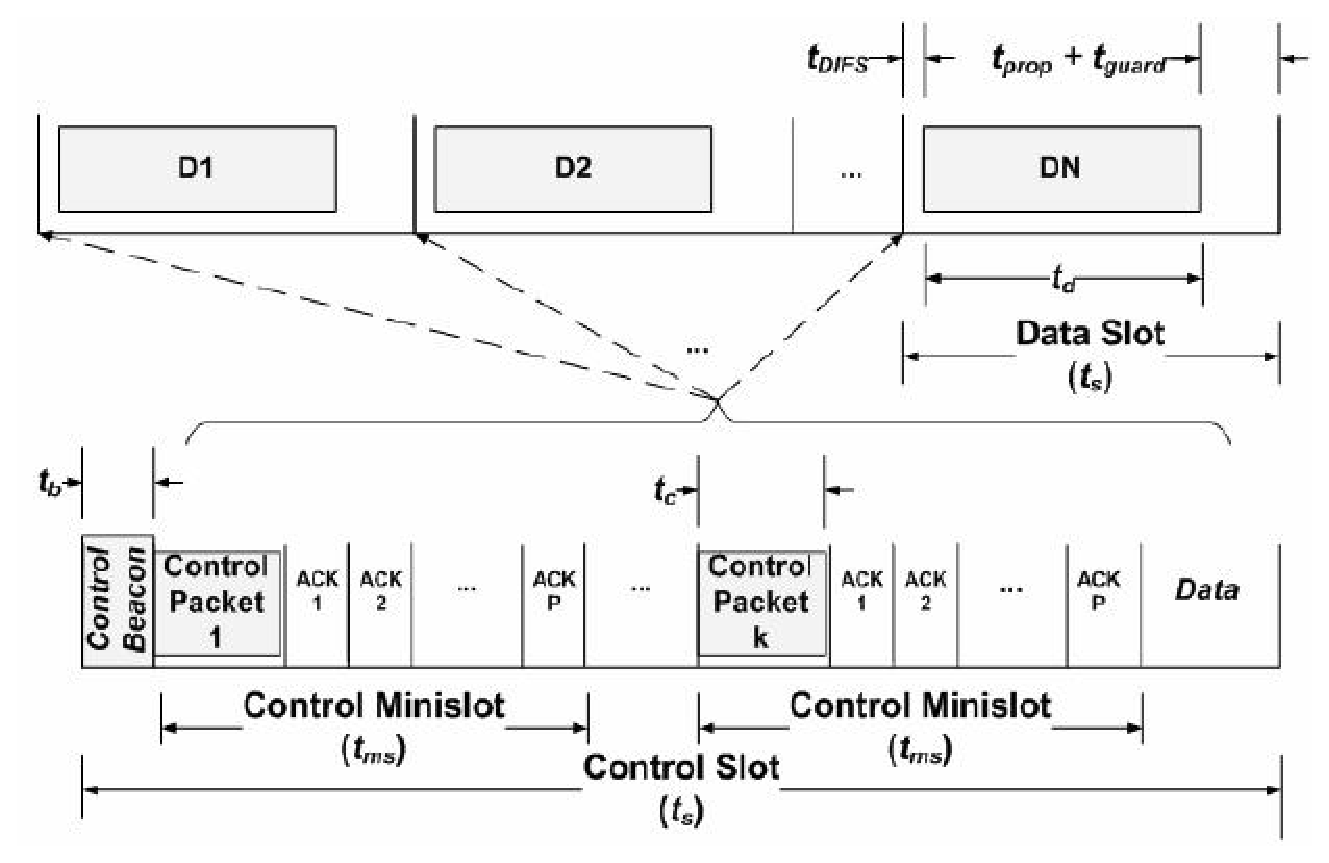
\includegraphics[scale=0.5]{imagens/cws-mac}
\end{frame}

\begin{frame}{Suporte aéreo para MAC \cite{20100312645920} \hyperlink{aerial_back}{\beamergotobutton{Voltar}}}
\hypertarget{aerial}{}
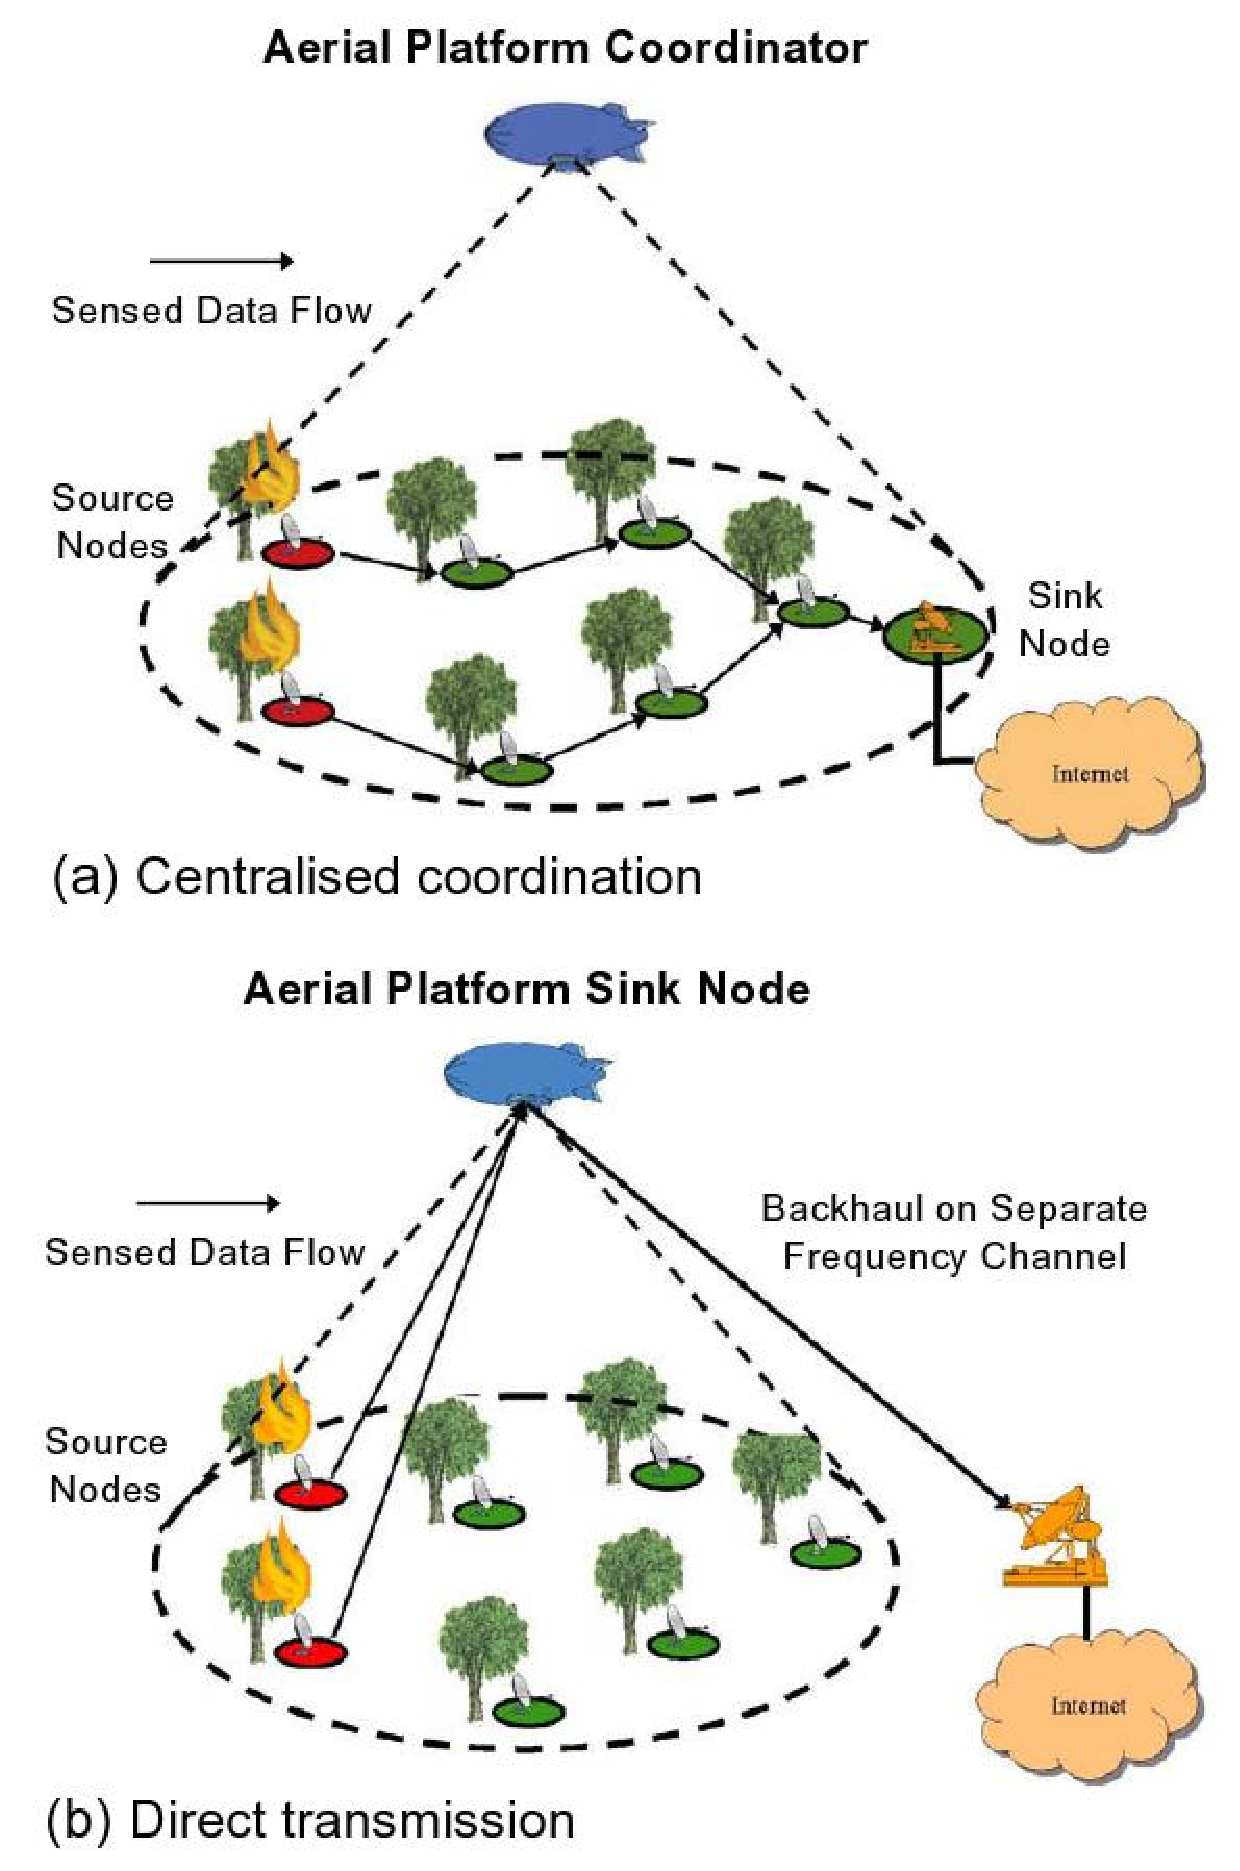
\includegraphics[scale=0.2]{imagens/aerial}
\end{frame}

\begin{frame}{Quadros para o APRMAC e APMAC \cite{20100312645920} \hyperlink{quadro_aerial_back}{\beamergotobutton{Voltar}}}
\hypertarget{quadro_aerial}{}
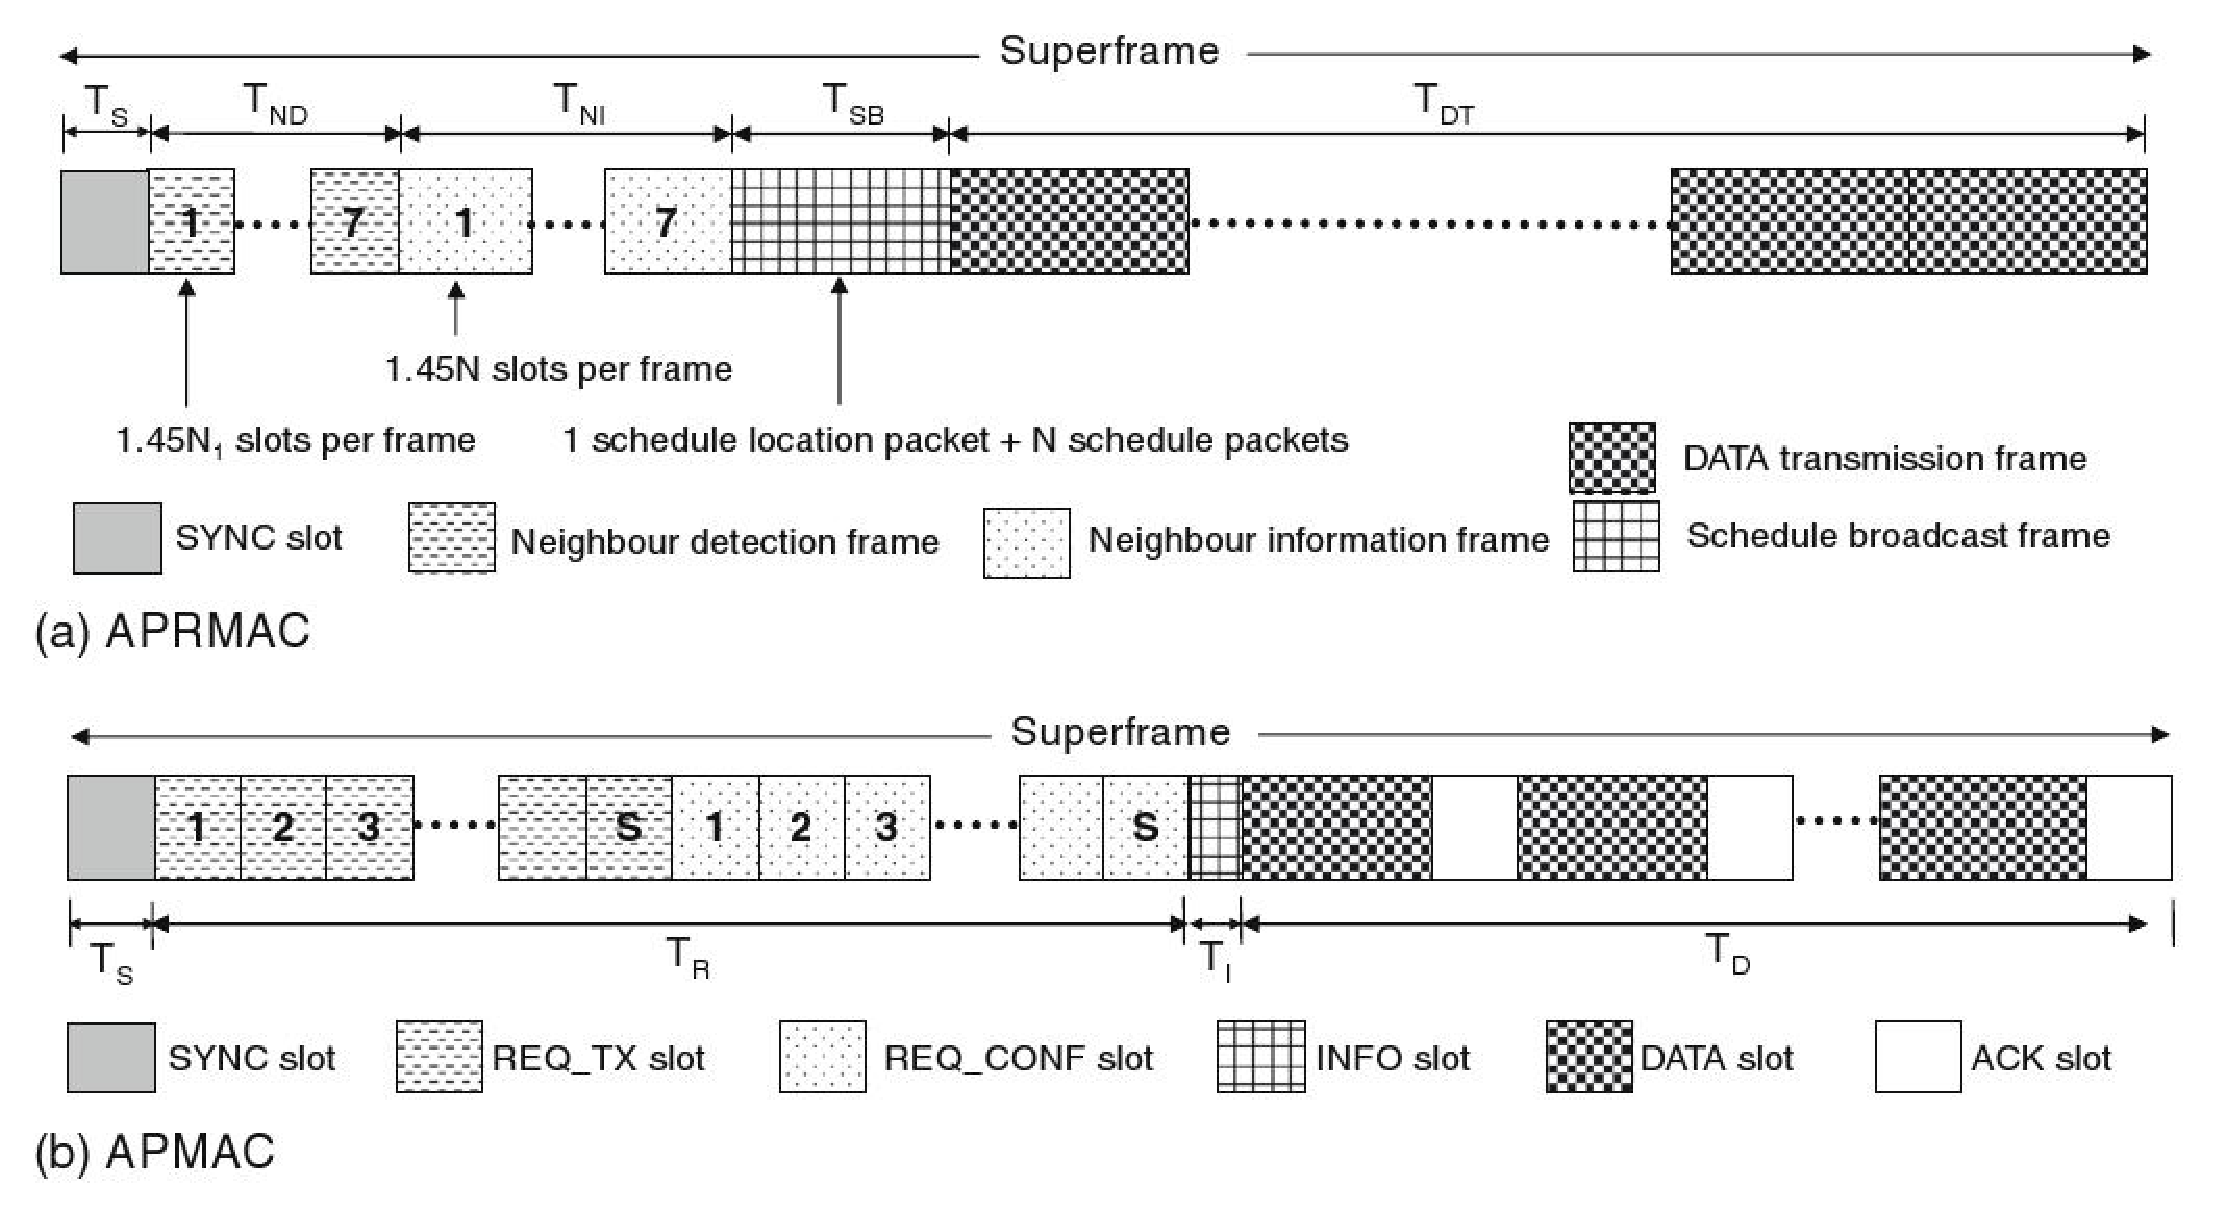
\includegraphics[scale=0.3]{imagens/quadro_aerial}
\end{frame}

\begin{frame}{Super-Quadro do G-MAC \cite{20093112234782} \hyperlink{quadro_g-mac_back}{\beamergotobutton{Voltar}}}
\hypertarget{quadro_g-mac}{}
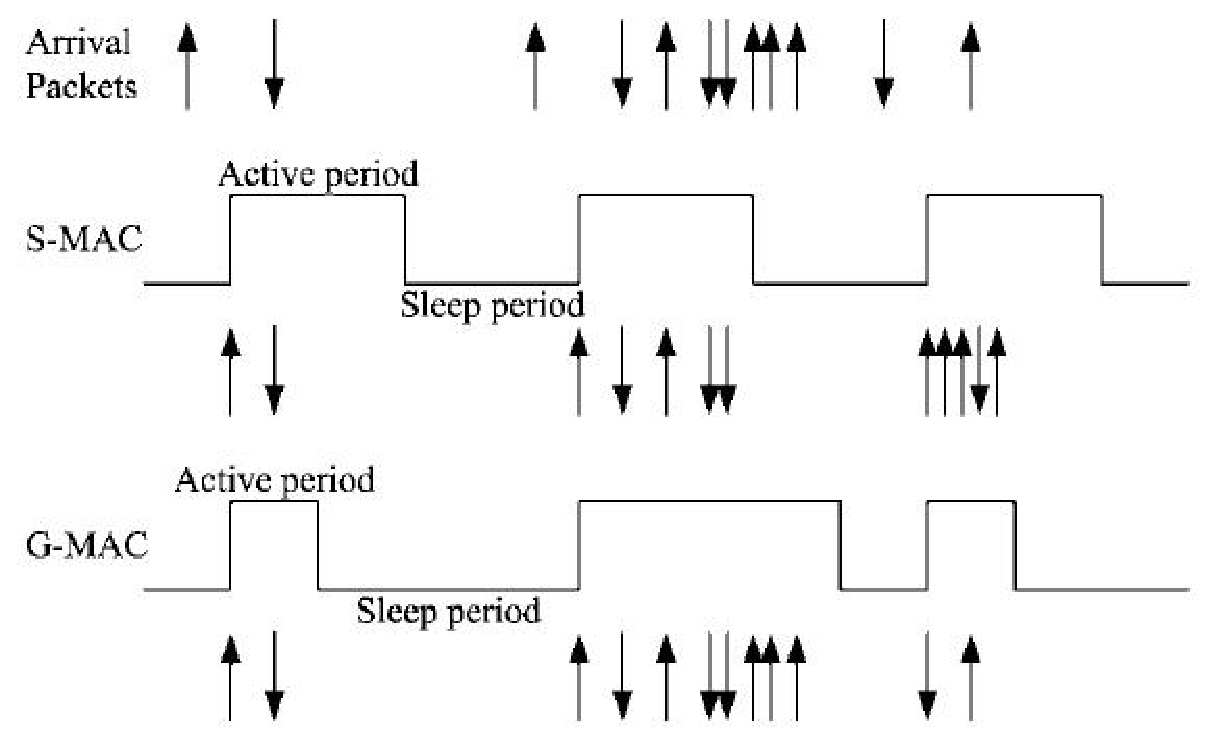
\includegraphics[scale=0.5]{imagens/quadro_g-mac}
\end{frame}

\begin{frame}{Troca de mensagens no CMAC \cite{20084511683228} \hyperlink{cmac_back}{\beamergotobutton{Voltar}}}
\hypertarget{cmac}{}
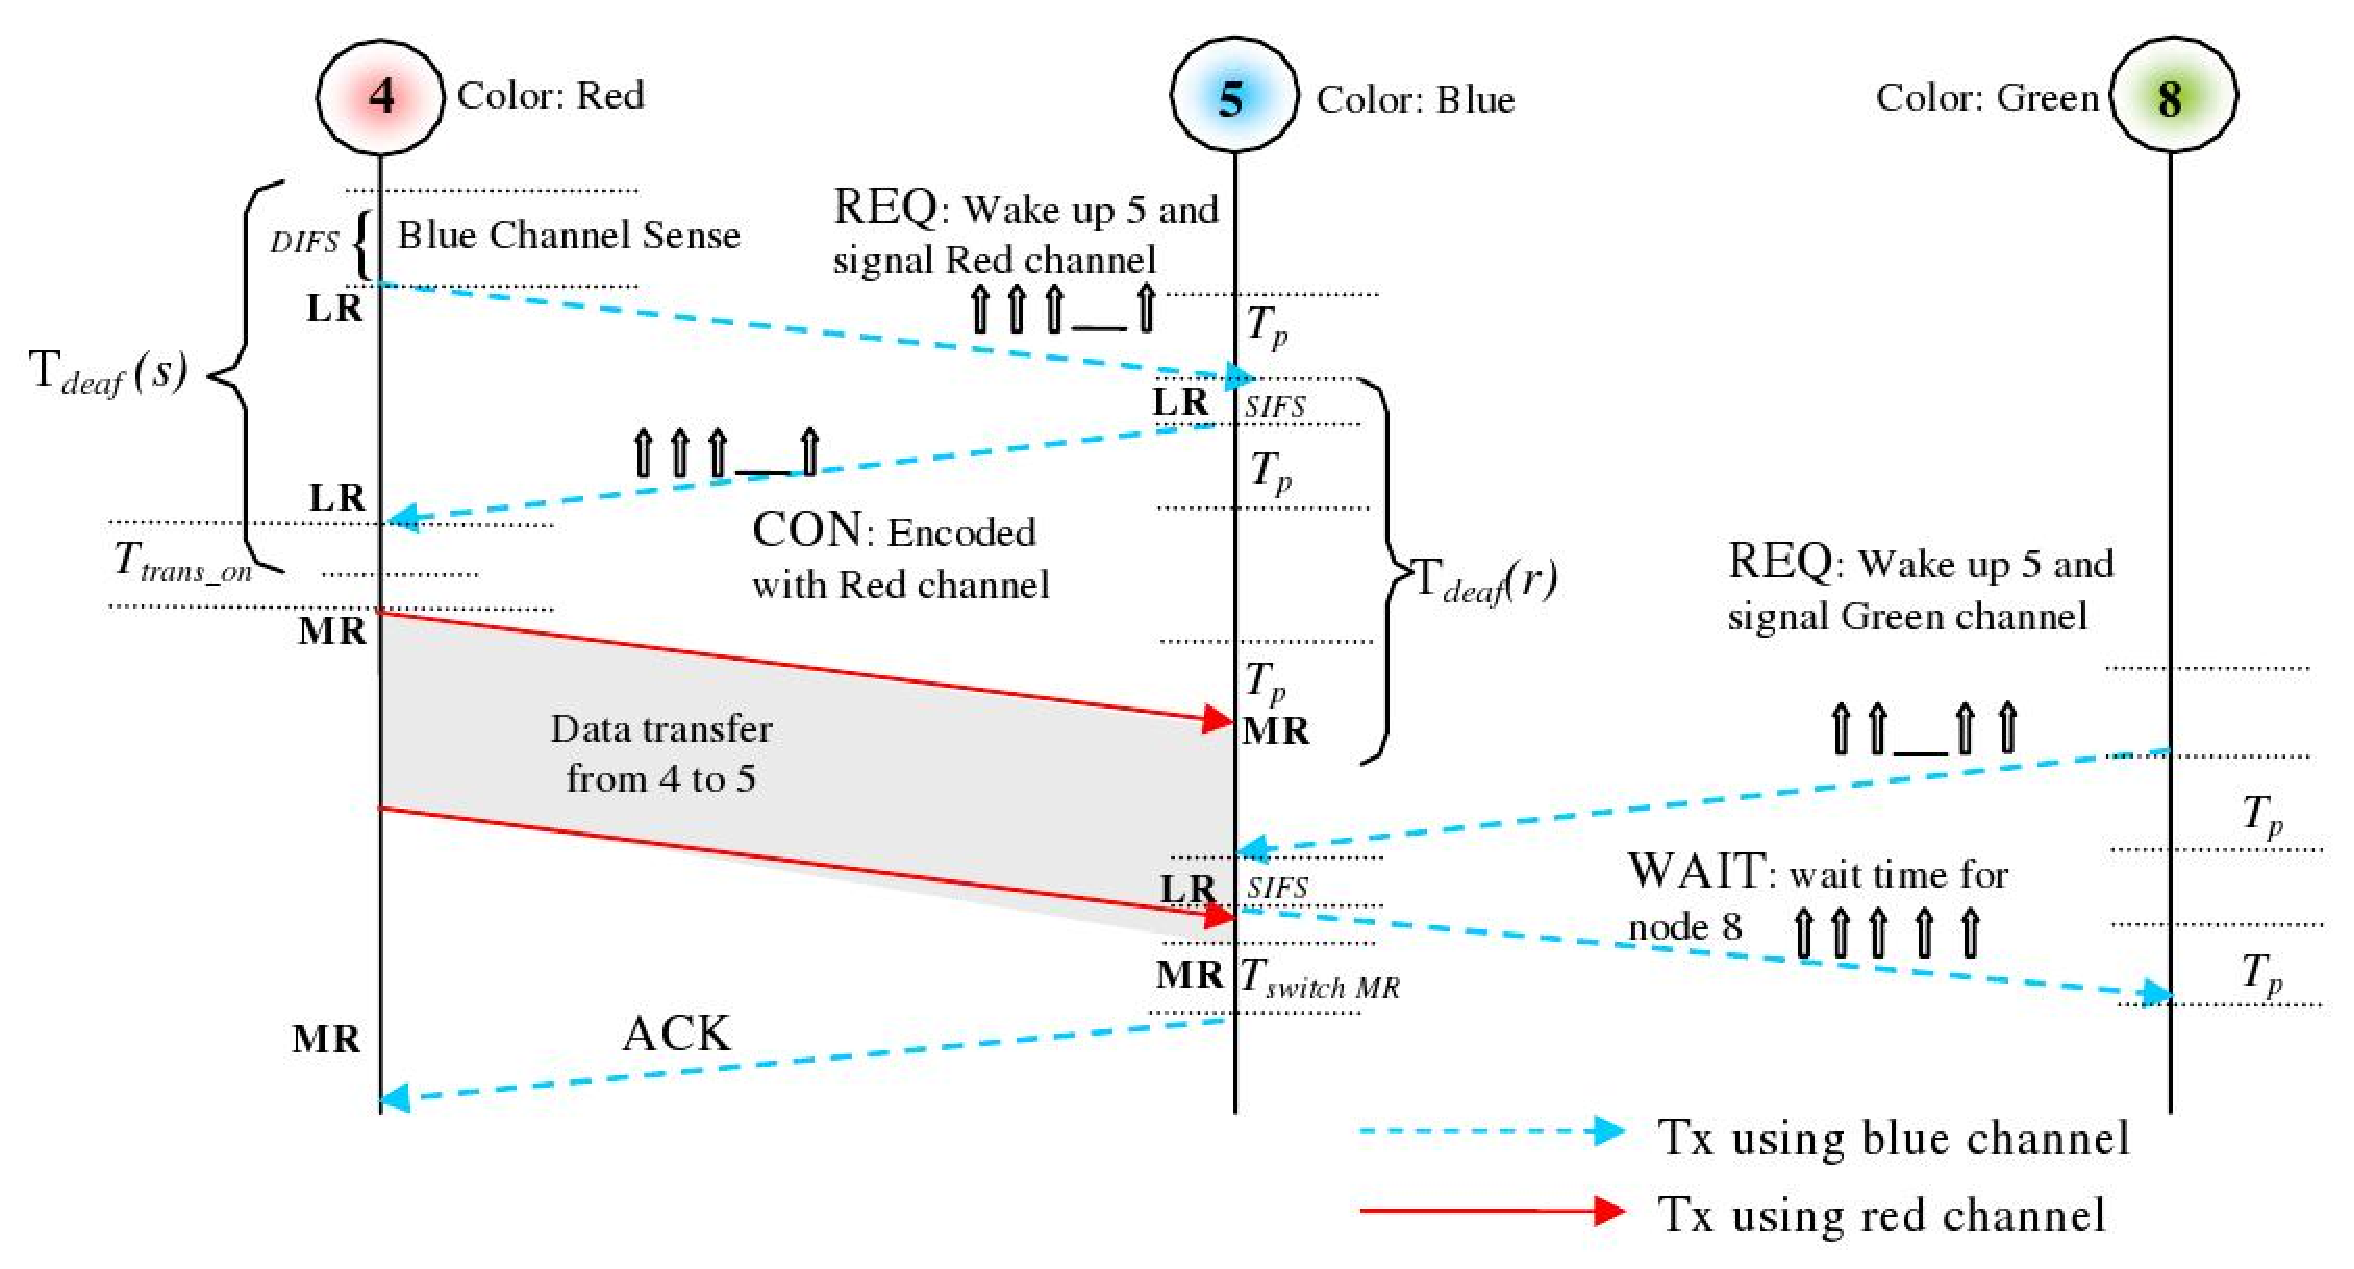
\includegraphics[scale=0.3]{imagens/cmac}
\end{frame}

\begin{frame}{Quadro do MCMAC \cite{20103113115754} \hyperlink{mcmac_back}{\beamergotobutton{Voltar}}}
\hypertarget{mcmac}{}
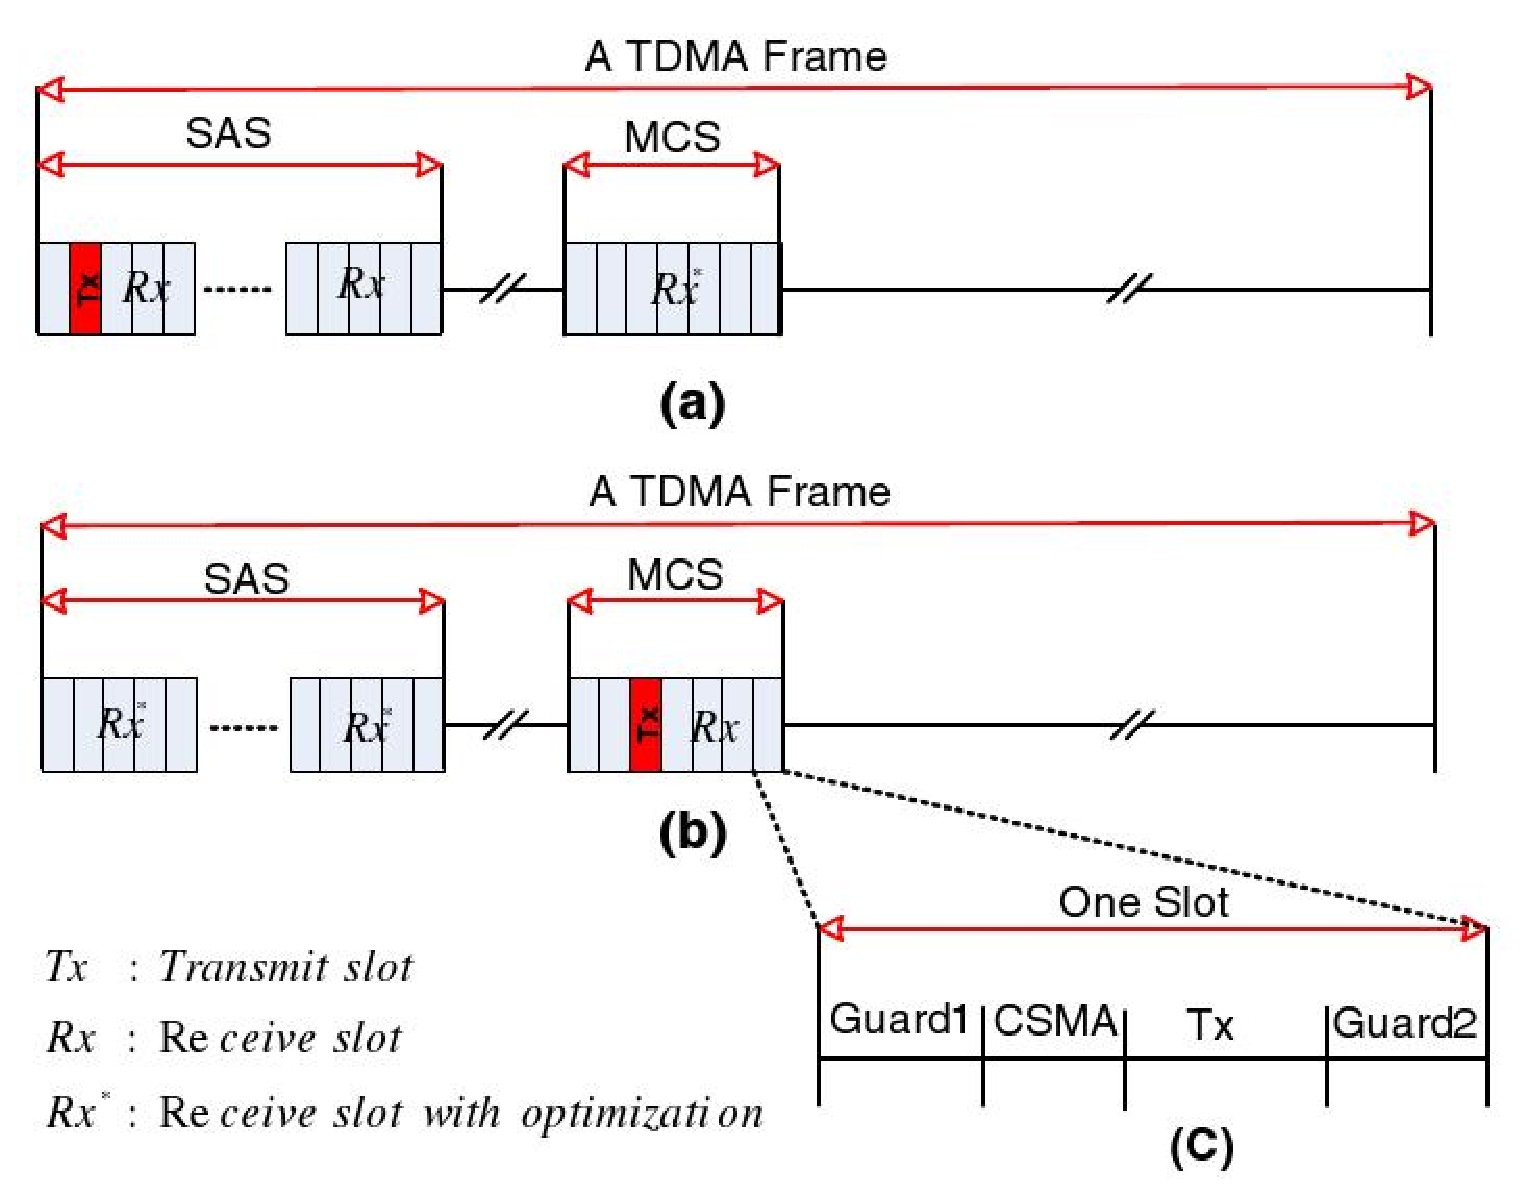
\includegraphics[scale=0.3]{imagens/mcmac}
\end{frame}

\begin{frame}{Árvore definida pelo MaCARI \cite{20092812183087} \hyperlink{macari_tree_back}{\beamergotobutton{Voltar}}}
\hypertarget{macari_tree}{}
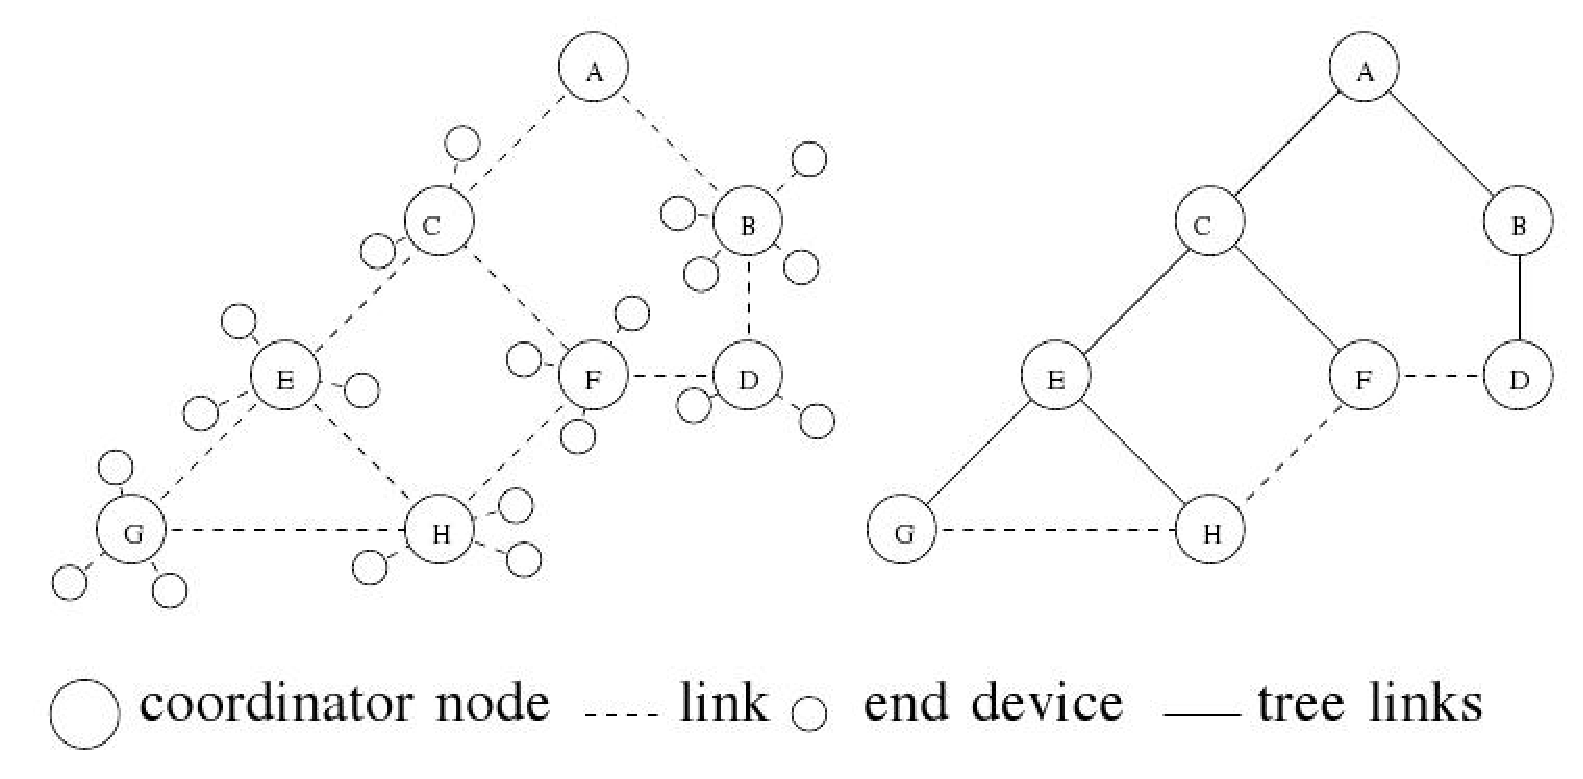
\includegraphics[scale=0.3]{imagens/macari_tree}
\end{frame}

\begin{frame}{Estrutura do EQ-MAC \cite{20092612148942} \hyperlink{eq-mac_back}{\beamergotobutton{Voltar}}}
\hypertarget{eq-mac}{}
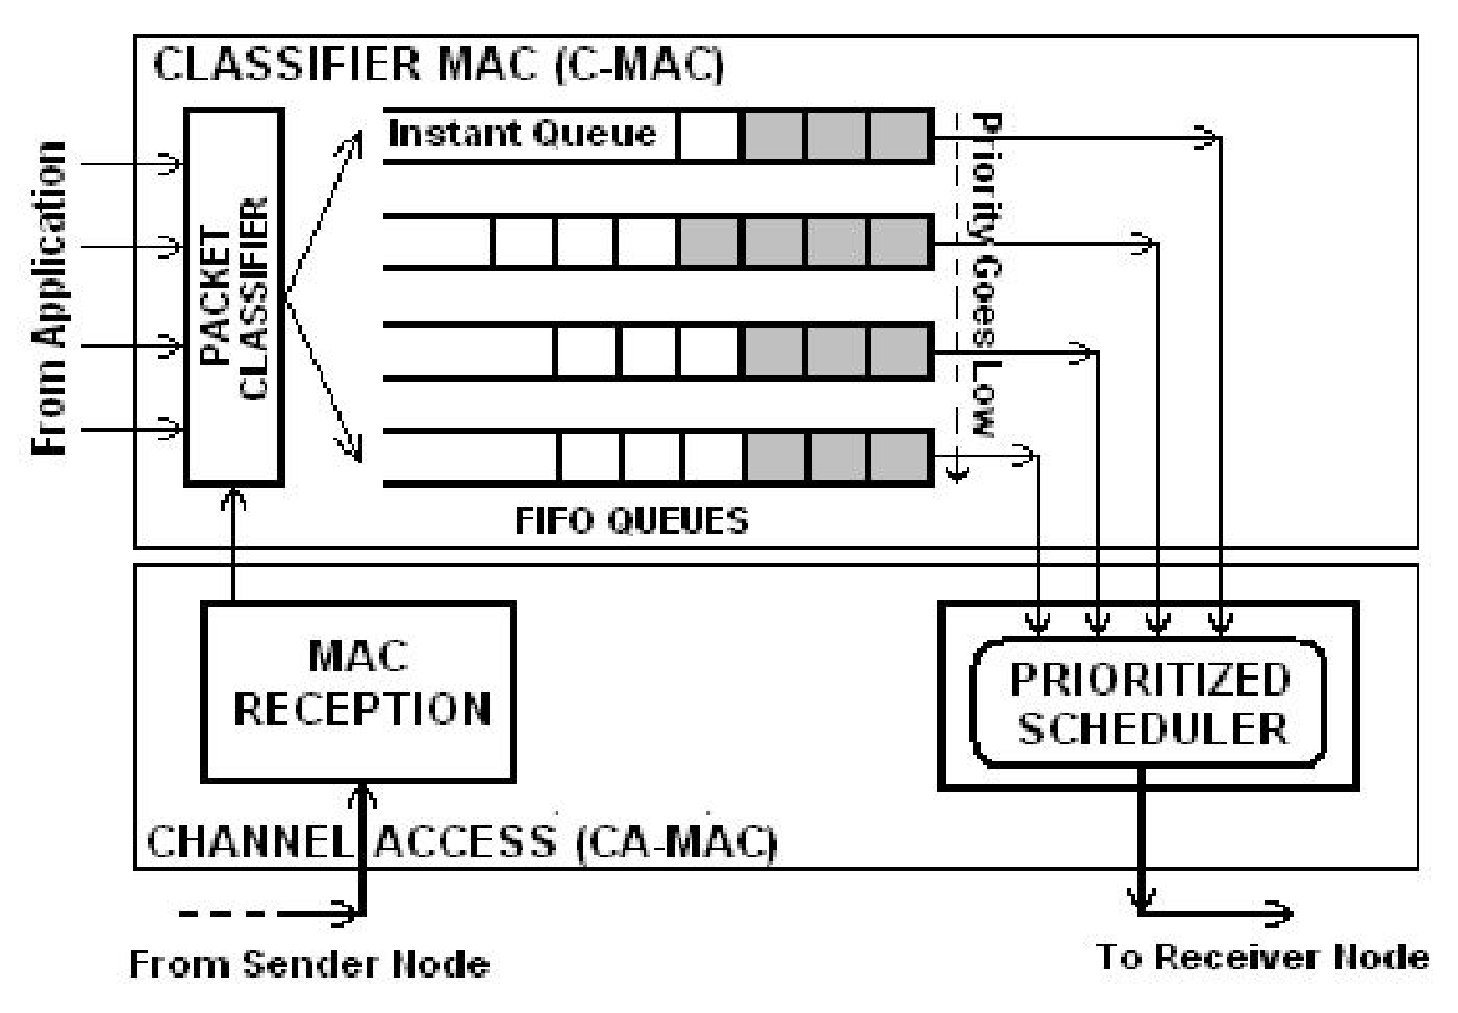
\includegraphics[scale=0.3]{imagens/eq-mac}
\end{frame}

\begin{frame}{Quadro do EQ-MAC \cite{20092612148942} \hyperlink{quadro_eq-mac_back}{\beamergotobutton{Voltar}}}
\hypertarget{quadro_eq-mac}{}
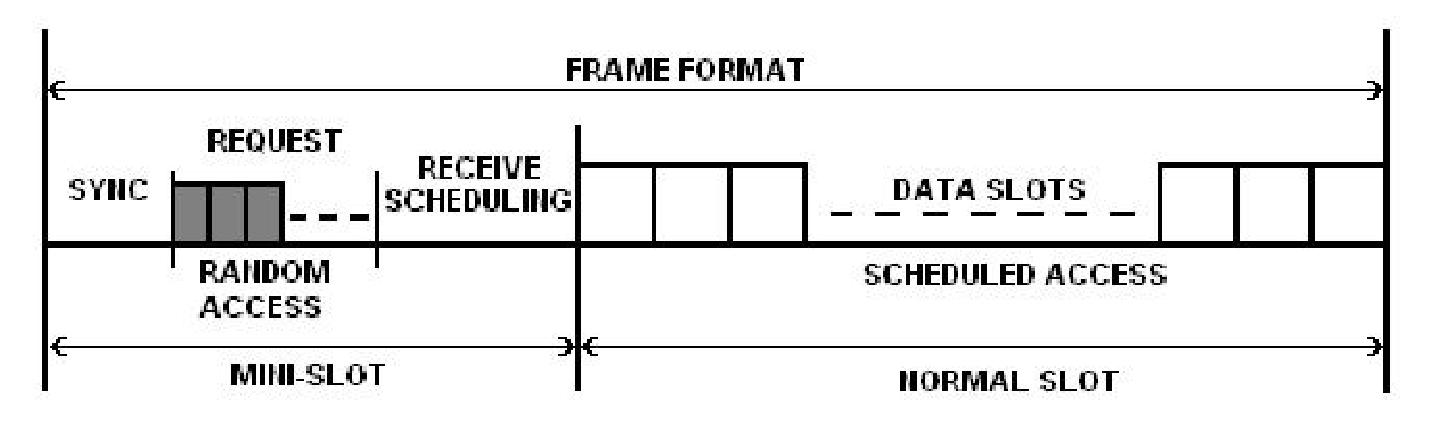
\includegraphics[scale=0.4]{imagens/quadro_eq-mac}
\end{frame}

\bibliographystyle{sbc}
\bibliography{projeto_final}

\end{document}


